    \section[État de l'art des outils d'analyse de robustesse]{État de l'art des outils d'analyse de robustesse pour l'injection de faute}
    \label{sec:soa-tools}

        Cette section propose un aperçu des outils existants pour l'évaluation de robustesse dans le cadre de la tolérance aux fautes et des attaques par injection de fautes. Elle vise aussi à proposer un ensemble de critères pour la comparaison de ces outils. L'état de l'art des outils et des techniques d'analyse pour l'injection de fautes a déjà fait l'objet de plusieurs articles de recherche \cite{kooli2014survey, Given/ICESS17, gangolli2022systematic} et de surveys \cite{Christofi/Phd13, Dureuil/Phd16, Heydemann/HDR17}. Les outils visant la tolérance aux fautes sont également considérés.        
        
        \begin{figure}[ht]\centering
          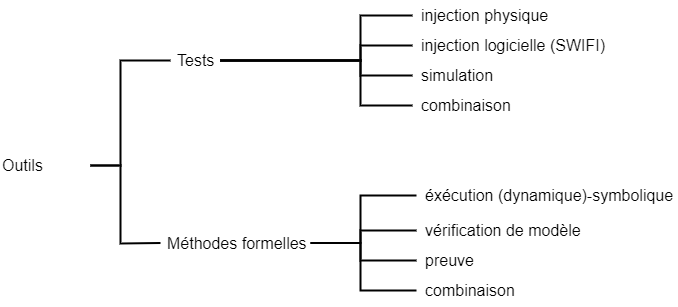
\includegraphics[scale=.45]{ch2-background/img/plan-soa-tools.drawio.png}
          \caption{Organisation et périmètre de l'état de l'art}
          \label{fig:soa-tools-scheme}
        \end{figure}
         
        La suite de cette section s'organise comme suit. La sous-section \ref{sec:soa-tools-carac} présente différents critères qui seront considérés pour la comparaison des outils. L'état de l'art est organisé en fonction de la technique d'analyse employée comme montré dans la figure \ref{fig:soa-tools-scheme}. Les sous-sections \ref{sec:soa-tools-test} et \ref{sec:soa-tools-formal} présentent respectivement les méthodes basées sur les tests et celles reposant sur les méthodes formelles.
        Enfin, la sous-section \ref{sec:soa-tools-conclusion} conclut cette section.
        
        \subsection{Caractéristiques des outils}
        \label{sec:soa-tools-carac}
     
            Différentes caractéristiques peuvent être considérées lorsqu'on s'intéresse à un outil d'analyse concernant les attaques en fautes.
            La figure \ref{fig:soa-tools-conclusion} présente une classification d'un ensemble de caractéristiques issus de la littérature et qui seront considéré dans cette section :
            
            \begin{figure}[hbt]\centering
              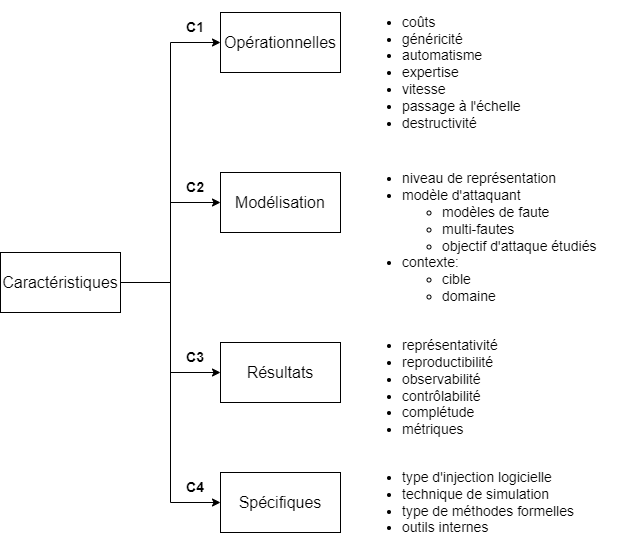
\includegraphics[scale=.55]{ch2-background/img/tools-carac.drawio.png}
              \caption{Classification des caractéristiques pour les outils d'analyse de robustesse contre les fautes}
              \label{fig:soa-tools-conclusion}
            \end{figure}
            
            \begin{itemize}
                \item[$\bullet$] \textbf{C1} Caractéristiques opérationnelles:
                \begin{itemize}
                    \item[-] \textit{Coûts}: regroupe les coûts liés au développement de l'outil en termes de moyens humains et de matériel ainsi que le niveau d'expertise requis par l'utilisateur pour l'utilisation de l'outil. 
                    \item[-] \textit{Généricité}: détermine à quel point l'outil est spécifique à un matériel ou une architecture donnée (on parlera à l'opposé de \textit{spécificité}).
                    \item[-] \textit{Automatisation}: niveau d'intervention de l'utilisateur requis.
                    \item[-] \textit{Expertise}: niveau d'expertise de l'utilisateur dans le domaine étudié ou la méthode d'analyse utilisée par l'outil. 
                    \item[-] \textit{Vitesse}:  comprend la vitesse d'exécution de l'outil pour une analyse ou encore le temps de mise en place nécessaire entre deux expérimentations. 
                    \item[-] \textit{Passage à l'échelle}: capacité de l'outil à analyser des programmes / systèmes complexes.
                    \item[-] \textit{Destructivité}: possibilité d'endommager le système étudié par l'analyse.
                \end{itemize}
                
                \item[$\bullet$] \textbf{C2} Caractéristiques liées à la modélisation:
                \begin{itemize}
                    \item[-] \textit{Niveau de représentation}: niveau de représentation de l'analyse (à ne pas confondre avec le niveau d'implémentation de l'outil).
                    \item[-] \textit{Modèle d'attaque}: modèles de faute supportés, support des fautes multiples et objectifs d'attaque étudiés.
                    \item[-] \textit{Contexte d'analyse}: 
                    \begin{itemize}
                        \item[$\circ$] \textit{Cible de l'analyse}: le type de système visé par l'analyse (programme, application, circuit, machines distribuées...).
                        \item[$\circ$] \textit{Domaine}: attaques en fautes, canaux auxiliaires ou fautes accidentelles.
                    \end{itemize}
                \end{itemize}                
                
                \item[$\bullet$]\textbf{C3} Caractéristiques liées aux résultats:
                \begin{itemize}
                    \item[-] \textit{Représentativité}: représentativité des résultats obtenus par rapport à une véritable attaque. 
                    \item[-] \textit{Reproductibilité}: détermine si les résultats obtenus peuvent facilement être reproduits. 
                    \item[-] \textit{Observabilité}: correspond à la capacité de la méthode d'observer l'effet des fautes injectées. 
                    \item[-] \textit{Contrôlabilité}: détermine le contrôle qu'offre la méthode sur les fautes qui seront injectées.
                    \item[-] \textit{Complétude}: couverture des exécutions fautées par l'analyse.
                    \item[-] \textit{Métriques}: métriques produites par l'outil.
                \end{itemize}
                
                \item[$\bullet$]\textbf{C4} Caractéristiques spécifiques: sous-classe de la technique d'analyse, technique d'implémentation.
            \end{itemize}
            
            Les caractéristiques suivantes, correspondant à des combinaisons de caractéristiques, seront aussi étudiées :
            \begin{itemize}
                \item \textit{Performance} (\textbf{C1}): passage à l'échelle et vitesse.
                \item \textit{Mise-en-place} (\textbf{C1}): regroupe les coûts lié au développement de l'outil en termes de moyens humains et de matériel et la destructivité.
                \item \textit{Accessibilité} (\textbf{C1}\&\textbf{C3}): regroupe les caractéristiques de l'expertise requise pour l'utilisateur, l'automatisme et la contrôlabilité.
            \end{itemize}
            
        \subsection{Outils basés sur le test}
        \label{sec:soa-tools-test}
        
            Cette sous-section s'intéresse aux outils basés sur le test, c'est-à-dire qui effectuent une sous-approximation des exécutions.
            Cette classe regroupe un grand nombre de techniques et d'outils:
            \begin{itemize}
                \item L'\textit{injection physique} (section \ref{sec:soa-tools-physic}) qui correspond à l'expérimentation en attaquant physiquement le système.
                \item L'\textit{injection logicielle} (section \ref{sec:soa-tools-swifi}) qui englobe tous les outils émulant l'effet des fautes physiques au niveau logiciel.
                \item La \textit{simulation}\footnote{Une partie de la littérature utilise le terme \textit{simulation} par opposition aux méthodes formelles \cite{kooli2014survey, Heydemann/HDR17}. Dans la suite de ce manuscrit, le mot \textit{simulation} ne sera pas employé en ce sens, parlant à la place d'\textit{outils basés sur les tests}.} (section \ref{sec:soa-tools-simu}) qui correspond aux outils exécutant le programme dans un simulateur dans lequel les fautes sont injectées.
            \end{itemize}        
        
            \subsubsection{Injection physique}
            \label{sec:soa-tools-physic}
            
                Une méthode d'injection de fautes physique (laser, glitches...) permet d'étudier le comportement du système soumis à des fautes. 
                Le terme \textit{injection de faute} a d'ailleurs émergé dans la littérature avant l'apparition des attaques par injection de fautes pour désigner des plateformes telles que MESSALINE \cite{Arlat/TSE90} ou encore RIFLE \cite{Madeira/DCC94}.
                Toute technique d'attaque par faute peut théoriquement être utilisée comme protocole de test physique pour un circuit.  
                
                \begin{figure}[hbt]\centering
                  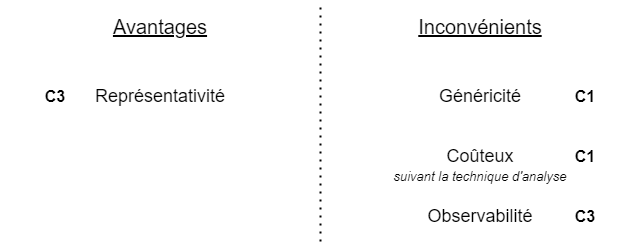
\includegraphics[scale=.45]{ch2-background/img/advantages-physics.drawio.png}
                  \caption{Caractéristiques de l'injection physique}
                  \label{fig:soa-tools-scheme-physic}
                \end{figure}
                
                La figure \ref{fig:soa-tools-scheme-physic} résume les avantages et inconvénients de ce type de techniques d'analyse. 
                L'indication $CI$ fait référence aux classes de caractéristiques présentées précédemment.
                L'injection physique à l'avantage d'obtenir des résultats très représentatifs sur la robustesse du programme puisque la faute est injectée directement sur le système à analyser et n'inclut donc pas d'étape intermédiaire ou d'abstraction pouvant fausser les résultats.
                L'observation et la caractérisation de la propagation des fautes observées sont difficiles et la mise en place d'un système d'observation peut introduire une perte de précision \cite{Faurax/Phd09, kooli2014survey}.
                
                La mise en place de tels bancs de test peut s'avérer coûteuse en fonction de la technique d'injection de fautes utilisée.
                Ces méthodologies d'analyse par injection physique sont souvent très spécifiques au système étudié par rapport à des approches plus haut niveau.
                De plus, certaines techniques d'injections destructrices peuvent endommager l'appareil étudié.
                Cependant, ces méthodes d'injections physiques sont utilisées pour la certification des composants sécurisés afin de démontrer la faisabilité d'une attaque.               
            
            \subsubsection{Injection au niveau logiciel (SWIFI)}
            \label{sec:soa-tools-swifi}
            
                Une autre technique très largement utilisée est la reproduction au niveau logiciel des fautes, ou de l'effet causé par des fautes au niveau de représentation considéré. 
                Cette technique désignée \gls{swifi} a émergé dès la fin des années 1980 \cite{Segall/FTCS88, Kanawati/FTCS92, Kao/TSE93} dans le milieu des fautes accidentelles pour ensuite se développer dans le domaine des attaques par injection de fautes jusqu'à aujourd'hui \cite{Georgakoudis/ICHPCNSA17}. 
                
                \paragraph{}         
                \gls{fiat} \cite{Segall/FTCS88} est l'un des premiers outils de type \gls{swifi} et a été proposé en 1988. Il vise l'analyse de systèmes distribués.
                Les fautes autorisées sont décrites par l'utilisateur à l'aide d'un langage spécifique et sont ensuite générées lors de la campagne d'expérimentation. Cet outil a notamment été utilisé pour analyser des fautes de type mise-à-zéro et mise-à-un d'octets et l'inversion de deux bits complémentaires \footnote{C'est-à-dire deux bits de valeurs différentes, afin d'éviter d'être détecté par un code correcteur d'erreur simple.} \cite{Barton/TC90}.   
                \gls{fine} \cite{Kao/TSE93}, est une plateforme d'analyse qui considère à la fois les fautes physiques et les fautes liées à des erreurs d'implémentation ou de conception logicielle, et qui vise à étudier la propagation des fautes dans un système d'exploitation.
                L'outil injecte les fautes au niveau logiciel à l'aide d'un noyau UNIX modifié traçant l'exécution et proposant des appels systèmes supplémentaires.
                Les fautes matérielles consistent en une mutation de données dans la mémoire, les registres ou les bus. 
                Les fautes logicielles sont implémentées en tant que modifications du programme binaire et incluent: données mal initialisées, assignation incorrectes, vérifications des cas d'erreurs incomplètes ou encore mauvaise sortie du programme.
                L'outil vise aussi à étudier comment les erreurs se propagent entre les différentes machines et les différents niveaux.
    
                L'outil \gls{define} \cite{Kao/FTPDS94} est une évolution de \gls{fine} qui supporte l'injection dans un système distribué. Celui-ci permet l'injection dans chaque machine, dans n'importe quelle application en mode utilisateur ou superviseur. 
                En plus des appels systèmes rajoutés et de la modification de l'image binaire du programme déjà utilisées dans \gls{fine}, \gls{define} utilise un handler modifié d'interruptions de l'horloge matérielle afin de contrôler l'injection des fautes dans les bus et la mémoire.
                Des expérimentations ont été menées sur un ensemble de 7 machines SunOS pouvant être fautées, l'une d'entre elles étant utilisée comme serveur. Les auteurs constatent que les erreurs sur le serveur se révèlent plus critiques en général que les fautes sur le client. 
                
                \gls{exfi} \cite{Benso/TODAES98} est un environnement d'injection de fautes qui utilise le \textit{trap execution mode} des microprocesseurs pour l'injection de fautes.
                Ainsi, \gls{exfi} ne nécessite pas de matériel spécialisé (comme FERRARI \cite{Kanawati/FTCS92} par exemple) ou la présence d'un système d'exploitation (comme les outils utilisant des traps logicielles type \gls{fine}).
                Une passe est utilisée pour réduire cet ensemble de fautes en fonction de règles spécifiques permettant d'écarter certaines fautes sans perdre en précision. 
                Ces règles visent à écarter les fautes qui n'auraient pas d'effet sur le système, seraient forcément détectées par un mécanisme de détection d'erreur et celles dont le comportement est déjà couvert par une autre faute de la liste.
                \gls{exfi} supporte un modèle de fautes temporaires de type bit-flip pouvant cibler les instructions, la mémoire et les registres.
                Une faute est caractérisée par le nombre d'instructions depuis le démarrage de l'application.
                
                \gls{llfi} \cite{Thomas/SELSE13, Lu/SQRS15}, proposé en 2013, est un outil pour la tolérance aux fautes travaillant sur la représentation intermédiaire \gls{llvm}.
                Celui-ci instrumente le programme à analyser et génère un exécutable pour l'injection de fautes et un exécutable de profilage déterminant quelles fautes vont être injectées.
                \gls{llfi} modélise des inversions de un ou deux bits et vise une douzaine d'instruction comprenant le calcul d'adresse (\texttt{load} et \texttt{store}) ou encore les opérations arithmétiques (\texttt{mul}, \texttt{fmul} etc.).
                L'outil ne considère que les fautes \textit{activées}, c'est-à-dire lorsque la donnée fautée est lue par le programme avant d'être écrasée par une autre instruction.
                Les auteurs constatent sur leurs expérimentations que certaines instructions (comme les instructions de comparaison)
                sont moins sensibles aux fautes que d'autres et que deux inversions augmentent le risque de crash sans augmenter le nombre d'erreurs de calcul non détectées.
    
                REFINE \cite{Georgakoudis/ICHPCNSA17} est une approche basée sur l'injection de fautes à la compilation qui vise à modéliser plus finement des comportements qui sont difficiles à capter au niveau d'une représentation intermédiaire (comme par exemple les prologues / épilogues de fonctions qui sont abstraits par l'IR LLVM).
                REFINE se situe dans le backend du compilateur et a ainsi accès aux instructions spécifiques (au prix de la portabilité).
                L'outil se place ainsi après toutes les passes d'optimisation afin d'éviter que le code injecté puisse être transformé par le compilateur. 
                REFINE se concentre sur un modèle de mutation d'opcode et d'opérande, ignorant les opcodes invalides.
                Les auteurs comparent leur approche à celle de \gls{llfi} qui s'applique également au niveau de l'IR \gls{llvm} et PINFI (qu'ils ont modifiés) qui travaille au niveau binaire sur différents programmes de calcul haute performance (\gls{hpc}).
                Ils indiquent que les performances et la précision de REFINE sont meilleures que celles de \gls{llfi} et égalent, voire dépassent dans certains cas, celles de PINFI. 
            
                \centerline{}
                \begin{table}[hbt]
                    {\tiny
                    \begin{center} 
                    \setlength\tabcolsep{4pt}
                    \begin{tabular}{|l|l|c|c|c|c|c|c|}
                    \hline
                    \multicolumn{1}{|c|}{Outil} & \multicolumn{1}{c|}{Niveau} & Technique & Modèle & Fautes & Cible & Oracle & FI \\ \hline
                    \begin{tabular}[c]{@{}l@{}}FIAT \\ \cite{Segall/FTCS88}\end{tabular} & Physique & \begin{tabular}[c]{@{}c@{}}materiel, OS\\ spécialisé\end{tabular} & \begin{tabular}[c]{@{}c@{}}mémoire\\ registres\\ communication\end{tabular} & 1 & \begin{tabular}[c]{@{}c@{}}système\\ distribué\end{tabular} & SDC & Non \\ \hline
                    \begin{tabular}[c]{@{}l@{}}Ferrari \\ \cite{Kanawati/FTCS92}\end{tabular} & Physique & \begin{tabular}[c]{@{}c@{}}software-trap\\ (syscall)\\ materiel spécialisé\end{tabular} & \begin{tabular}[c]{@{}c@{}}mémoire, registre\\ remplacement inst.\\ fautes permanentes\end{tabular} & 1 & \begin{tabular}[c]{@{}c@{}}système\\ distribué\end{tabular} & SDC & Non \\ \hline
                    \begin{tabular}[c]{@{}l@{}}DEFINE \\ \cite{Kao/FTPDS94}\end{tabular} & UNIX & \begin{tabular}[c]{@{}c@{}}kernel modifié\\ interrupt modifiées\end{tabular} & \begin{tabular}[c]{@{}c@{}}CPU (ALU, cache,\\ decoder, reg, bus), \\ communication\\ fautes de design\end{tabular} & 1 & \begin{tabular}[c]{@{}c@{}}système\\ distribué\end{tabular} & SDC & Non \\ \hline
                    \begin{tabular}[c]{@{}l@{}}Xception \\ \cite{Carreira/IEEE98}\end{tabular} & CPU & \begin{tabular}[c]{@{}c@{}}fonctionnalité\\ CPU\end{tabular} & \begin{tabular}[c]{@{}c@{}}flips, sa1, sa0, bit mask\\ CPU registre bus\end{tabular} & 1 & application & SDC & Non \\ \hline
                    \begin{tabular}[c]{@{}l@{}}EXFI \\ \cite{Benso/TODAES98}\end{tabular} & µkernel & software-trap & \begin{tabular}[c]{@{}c@{}}bitflip\\ (mem / reg)\end{tabular} & 1 & application & SDC & Non \\ \hline
                    \begin{tabular}[c]{@{}l@{}}LLFI \\ \cite{Thomas/SELSE13}\end{tabular} & LLVM & compilation & \begin{tabular}[c]{@{}c@{}}flip ALU\\ store / load\end{tabular} & 1 & application & SDC & Non \\ \hline
                    \begin{tabular}[c]{@{}l@{}}REFINE \\ \cite{Georgakoudis/ICHPCNSA17}\end{tabular} & LLVM & compilation & \multicolumn{1}{l|}{bit-flip sur opérandes} & 1 & \multicolumn{1}{l|}{\begin{tabular}[c]{@{}l@{}}application\\ (HPC)\end{tabular}} & SE & Non \\ \hline
                    \end{tabular}
                \end{center}
                }       
                \caption{Comparaison de quelques outils de type SWIFI \label{tbl:tools-swifi}}
                \end{table}

                \paragraph{}
                La table \ref{tbl:tools-swifi} présente une comparaison de quelques outils de type \gls{swifi}.
                La colonne \textit{Niveau} indique le niveau d'abstraction auquel se place l'outil.
                La colonne \textit{Technique} correspond à la méthode utilisée pour émuler les fautes au niveau logiciel.
                La colonne \textit{Modèle} précise les modèles de faute supportés et la colonne \textit{Faute} la limite de faute pour les attaques.
                La colonne \textit{Cible} correspond au type de système étudié par l'outil (système distribué, application etc.).
                La colonne \textit{Oracle} indique le type de propriété de sécurité ou de sûreté étudiée par l'outil. Ici \textit{SDC} fait référence aux corruptions silencieuses de données.
                Enfin, la colonne \textit{FI} détermine si l'outil vise le milieu des attaques par injection de fautes ou celui des fautes accidentelles (ici tous).
                
                La figure \ref{fig:soa-tools-scheme-swifi} résume les avantages et inconvénients des outils \gls{swifi} comparés aux méthodes d'injection physiques. L'injection logicielle est généralement moins coûteuse, plus facile à mettre en place et plus générique.
                L'observabilité est également supérieure avec les approches d'injection logicielle, qui peuvent tirer partie de certaines technologies comme les exceptions matérielle (\gls{exfi}) \cite{Benso/TODAES98}.
                
                \begin{figure}[htpb]\centering
                  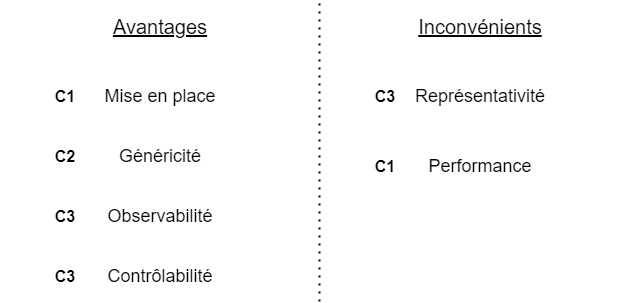
\includegraphics[scale=.41]{ch2-background/img/advantages-swifi.drawio.png}
                  \caption{Caractéristiques des méthodes SWIFI comparées à l'injection physique}
                  \label{fig:soa-tools-scheme-swifi}
                \end{figure}
                
                La sur-couche logicielle pour émuler la faute offre une représentativité moindre par rapport à l'injection physique et peut aussi ajouter une surcharge qui diminue les performances. Cette perte de précision dépend de la technique d'injection logicielle utilisée et des optimisations ont été développées qu'il s'agisse de représentativité ou de performance \cite{Lu/SQRS15, Georgakoudis/ICHPCNSA17}.
    
            \subsubsection{Outils basés sur la simulation}
            \label{sec:soa-tools-simu}
            
                La simulation désigne les outils qui effectuent une exécution sur un système simulé, sans exécuter directement sur le matériel étudié. 
                Les caractéristiques de l'outil dépendent alors en grande partie de la modélisation du système dans le simulateur.
                
                \paragraph{} 
                Depend \cite{Goswami/TC97} est un simulateur qui vise à prendre en compte les interactions entre les différents composants d'un système complexe en cas de fautes accidentelles.
                L'outil modélise le système en C++ afin de simuler des fautes au niveau des portes logiques. 
                Depend est capable de simuler des fautes sur la mémoire (bit-flip) et dans les communications (paquet perdu, corruption...). Les fautes sont décrites par l'utilisateur en C++ également.
                
                SINJECT \cite{Zarandi/DFTVS03} est un outil qui analyse la robustesse face aux fautes accidentelles au niveau de la représentation \gls{vhdl} et Verilog. 
                Il permet d'injecter un large nombre de fautes physiques au niveau des données et du circuit. Ceux-ci sont introduits dans le système Verilog à partir d'une description utilisateur. L'injection en \gls{vhdl} est faite avec la technique mutant-saboteurs.
                L'outil profite du mode combiné \gls{vhdl}/Verilog permettant de profiter de la représentativité de Verilog et de la description \gls{vhdl}.
                SINJECT s'intéresse à des objectifs d'attaque de tolérance aux fautes sur les traces simulées.
                
                \gls{pafi} \cite{Faurax/CSS06, Faurax/Phd09} est un outil étudiant les fautes au niveau du circuit utilisant la modélisation Verilog et \gls{vhdl}. 
                Il vise à vérifier l'absence de fuite de données secrètes dans le cadre d'attaques en multi-fautes au niveau circuit.
                L'outil s'appuie sur le simulateur Cadence NCSim (un outil propriétaire de STMicroelectronics) et utilise le fichier de commandes du simulateur pour contrôler les fautes à injecter.
                Une pondération basée sur des critères définis en fonction du modèle de faute permet de sélectionner les fautes à simuler (bit-flip sur les bascules ou faute sur les délais dans le circuit), ce qui permet un meilleur passage à l'échelle en multi-fautes.
                Par ailleurs, l'outil prend en compte les mécanismes de détection et indique les faux-positifs, faux-négatifs, attaques non détectées et attaques détectées.
                L'outil se veut extensible et générique en proposant un moyen de définir le modèle de circuit et les modèles de faute.
                
                \begin{sloppypar}   
                Celtic \cite{Dureuil/Phd16, Werner/Phd22} est un simulateur au niveau binaire développé en C++ qui permet de simuler des fautes au niveau de l'\gls{isa} et de l'architecture.
                Celtic supporte les fautes comme le saut d'instruction, la corruption du cache d'instruction \cite{Riviere/HOST15} et les attaques sur les données sur les registres, la mémoire et le décodage des instructions. L'outil supporte également les fautes multiples, ceci étant facilité par la parallélisation des simulations.
                L'objectif d'attaque est exprimé dans le programme et évalué pour chaque trace simulée afin de récupérer les attaques réussies.
                Celtic propose un langage de spécification d'architecture (GISL) permettant d'adapter facilement l'outil à différentes architectures. 
                \end{sloppypar}   
            
                \begin{table}[h]
                {\tiny
                \begin{center}                
                \setlength\tabcolsep{3.9pt}
                    \begin{tabular}{|l|l|l|l|l|l|l|l|l|}
                    \hline
                    Outil & Niveau & Implem & Simu type & Modèle & Fautes & Cible & Oracle & FI \\ \hline
                    FOCUS \cite{Choi/TC92} & Physique & VLSI & externe & porte logiques & X & \begin{tabular}[c]{@{}l@{}}systèmes\\ distribués\end{tabular} & SDC & Non \\ \hline
                    Depend \cite{Goswami/TC97} & \begin{tabular}[c]{@{}l@{}}Circuit\\ µ-arch\end{tabular} & C++ & intégrée & \begin{tabular}[c]{@{}l@{}}circuit\\ communication\\ mem.\end{tabular} & 1 & \begin{tabular}[c]{@{}l@{}}systèmes\\ distribués\end{tabular} & SDC & Non \\ \hline
                    SINJECT \cite{Zarandi/DFTVS03} & \begin{tabular}[c]{@{}l@{}}Verilog /\\ VHDL\end{tabular} & \begin{tabular}[c]{@{}l@{}}Verilog /\\ VHDL\end{tabular} & intégrée & circuit & 1 & application & SDC & Non \\ \hline
                    PAFI  \cite{Faurax/CSS06} & Circuit & \begin{tabular}[c]{@{}l@{}}Verilog /\\ VHDL\end{tabular} & externe & \begin{tabular}[c]{@{}l@{}}bit-flip\\ délais\end{tabular} & X & \begin{tabular}[c]{@{}l@{}}Verilog /\\ VHDL\end{tabular} & \begin{tabular}[c]{@{}l@{}}SC\\ exploit-\\ abilité\\ blocage\end{tabular} & Oui \\ \hline
                    CELTIC  \cite{Werner/Phd22} & x86 & C++ & intégrée & \begin{tabular}[c]{@{}l@{}}data (reg, mem)\\ cache, saut, rejeu\end{tabular} & X & x86 & \begin{tabular}[c]{@{}l@{}}oracle\\ logiciel\end{tabular} & Oui \\ \hline
                    \end{tabular} \end{center}
                }            
                \caption{Comparaison de quelques outils de simulation \label{tbl:tools-simu}}
                \end{table}

                La table \ref{tbl:tools-simu} présente une comparaison de plusieurs outils de simulation.
                Les colonnes \textit{Niveau}, \textit{Modèle}, \textit{Cible}, \textit{Oracle} et \textit{FI} ont la même signification que pour la table des outils \gls{swifi}. 
                La colonne \textit{Fautes} indique la limite de faute, le symbole "X" indiquant le support des fautes multiples.
                La colonne \textit{Implem} correspond au niveau auquel l'outil est implémenté (ce qui peut être différent du niveau de représentation étudié par l'outil).
                La colonne \textit{Simu type} indique si l'injection de fautes est intégrée au simulateur ou si les fautes sont émulées pour un simulateur existant.
                
                La figure \ref{fig:soa-tools-scheme-simu} présente les avantages et inconvénients de la simulation par rapport aux méthodes d'analyse présentées précédemment.
                En fonction de la modélisation du système par le simulateur, la généricité de l'outil et la représentativité des résultats peuvent être très variables. La généricité de l'approche est en relation directe avec le niveau de représentation du simulateur mais dépend aussi des choix du simulateur, GISL permettant par exemple une portabilité d'architecture pour CELTIC.
                Le développement d'un simulateur pour un système donné est le plus généralement coûteux par rapport à l'injection logicielle, mais le simulateur peut être disponible avant le matériel simulé ce qui a un intérêt dans le cycle de développement. 
                Les performances sont souvent moins bonnes qu'avec les approches citées précédemment.
    
                \begin{figure}[hbt]\centering
                  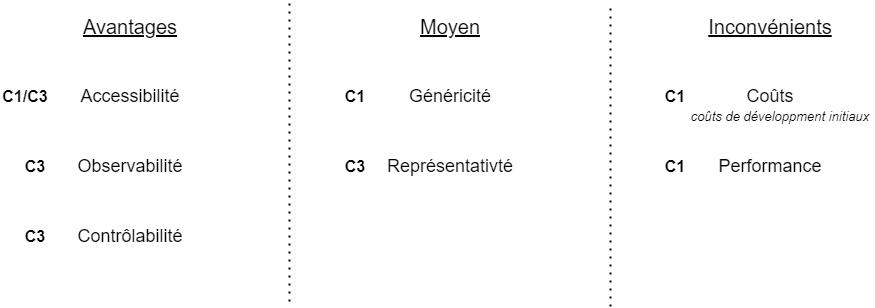
\includegraphics[scale=.56]{ch2-background/img/advantages-simu.drawio.png}
                  \caption{Comparaison des outils de simulation par rapport aux méthodes précédentes}
                  \label{fig:soa-tools-scheme-simu}
                \end{figure}
                
                On peut également opposer les simulateurs qui prennent en compte les fautes (comme Depend ou Celtic par exemple) et les implémentations qui s'appuient sur un simulateur existant et suivent alors le modèle \gls{swifi} en reproduisant l'effet d'une faute dans le modèle en question (tels que \gls{pafi}). 
                L'observabilité et le contrôle de la description des fautes est souvent bonne pour ce type de techniques puisque l'accès au système est plus facile sur un simulateur que sur le matériel et le simulateur peut accéder à des parties plus bas niveau du système que pour l'injection logicielle.
                
        \subsection{Méthodes formelles}
        \label{sec:soa-tools-formal}
            
            Les outils cités précédemment, à quelques exceptions près (comme Depend), comparent les exécutions fautées obtenues à une exécution de référence (\textit{golden run}). Pour chaque expérimentation ou simulation, les entrées du programme ou du système sont fixées ainsi que les fautes devant être injectées. Ces outils tentent de couvrir le maximum d'attaques en effectuant une série de tests avec différents paramètres pour les entrées et les fautes.
            
            Si différentes solutions ont été développées parmi ces outils basés sur les tests, comme réduire l'espace de faute \cite{Benso/TODAES98}, sélectionner un seul représentant pour une attaque \cite{Schmidt/Austrochip07} ou bien encore le développement de modèle plus haut niveau faisant abstraction de certains comportements, la couverture de ces outils est encore loin d'être parfaite. C'est pourquoi des solutions basées sur les méthodes formelles ont émergées afin d'obtenir une plus grande couverture des exécutions (des entrées et des fautes) ou bien de prouver des propriétés générales sur un programme ou un circuit, pour toutes fautes et pour toutes les entrées d'un modèle donné.
            
            \begin{figure}[hbt]\centering
              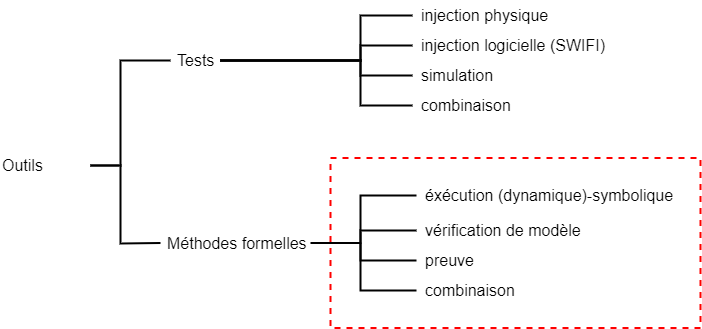
\includegraphics[scale=.45]{ch2-background/img/plan-soa-tools-formal.drawio.png}
              \caption{Outils basés sur les méthodes formelles}
              \label{fig:soa-tools-scheme-plan}
            \end{figure}
                
            La figure \ref{fig:soa-tools-scheme-plan} est un rappel du plan de la section \ref{sec:soa-tools} mettant en évidence les approches basées sur les méthodes formelles. 
            Ces outils basés peuvent parfois être rapprochés des techniques de simulation, dans le sens où le système n'est pas exécuté directement sur le matériel, mais analysé statiquement. C'est le cas pour l'exécution symbolique où le moteur d'exécution simule une exécution (ou plus exactement un ensemble d'exécutions) dans un modèle donné.
            De la même manière, certaines approches se rapprochent des méthodes de types \gls{swifi}, lorsque l'effet des fautes est mis en place dans le programme ou sa représentation, afin d'être fournies à un outil d'analyse formelle n'ayant pas de représentation pour les fautes \cite{Potet/ICST14, Le/DATE18}. 
            Les analyses formelles peuvent être appliquées à différents niveaux de représentation, en allant du niveau source aux représentations bas niveau comme le \gls{rtl} ou la spécification du circuit par exemple.             
            
            \paragraph{} 
            En 2007, Larsson et al. \cite{Larsson/VERIFY07} proposent une méthode appelée \textit{symbolic fault injection}. Ils présentent un outil d'analyse dans le cadre de la tolérance au fautes d'un programme source en Java et qui se base sur l'analyse formelle et l'exécution symbolique.
            Une instruction spécifique \texttt{inject(location);} est utilisée afin de spécifier que la zone mémoire \texttt{location} (variable, attribut etc.) peut être fautée. Leur implémentation utilise un modèle de bit flip sur les données et repose sur l'outil Key \cite{Ahrendt/Springer05}, une plateforme d'analyse formelle pour Java qui propose des fonctionnalités pour la vérification statique étendue, l'exécution symbolique, la vérification déductive et la spécification formelle.
            Des règles spécifiques ont été ajoutées dans Key pour simuler l'effet d'une faute dans l'état symbolique du programme.
            L'outil n'est cependant pas totalement automatique puisque l'utilisateur est sollicité pour spécifier les invariants de boucles par exemple.
            
            \textit{SymplFIED} \cite{Pattabiraman/DSN08}, est un outil d'évaluation reposant sur l'exécution symbolique et le model checking \cite{Pattabiraman/TC12}.
            L'outil prend en entrée un modèle de faute et un programme en assembleur qu'il transforme en un langage assembleur générique de type \gls{risc}.
            Cette représentation est implémentée avec le système Maude \cite{Clavel/ENTCS96, clavel2002maude} qui est un outil permettant la vérification de propriété sur un modèle et qui se base sur la \textit{rewritting logic}.
            SymplFIED supporte les fautes transitoires de un ou plusieurs bits dans le décodeur d'instruction, l'unité de calcul, les bus d'adresses et de données ou encore le fetch d'instruction, en faute unique.
            L'outil définit une procédure de modélisation de chaque type de faute sur le modèle machine dans Maude ainsi que des règles de propagation des erreurs entre les différents modules modélisés. Une erreur est représentée par un symbole \texttt{err} qui est propagé au fur et à mesure de l'exécution symbolique du programme.
            En plus de cela, l'outil vise à énumérer les cas d'erreurs qui ne sont pas détectées par des \textit{détecteurs}.
            La modélisation dans Maude fait quelques hypothèses comme l'absence d'erreur dans les détecteurs ou le fait que tout accès à une mémoire non initialisée donnera lieu à une exception et certaines opérations comme la multiplication ne sont pas exécutées symboliquement \cite{Pattabiraman/TC12}. 
            
            \textit{Lazart} \cite{Potet/ICST14} est un outil d'analyse de robustesse de programme sur la plateforme \gls{llvm} qui repose sur l'exécution symbolique effectuée par l'outil KLEE \cite{Cadar/OSDI08}. Lazart propose le modèle de l'inversion de test et chaque faute possible dans le programme est représentée par un booléen symbolique ce qui permet de générer les différents chemins d'attaque. 
            L'objectif d'attaque est défini à l'aide d'une propriété d'atteignabilité (par exemple le bloc d'authentification dans le programme \texttt{verify\_pin}) et les auteurs utilisent un algorithme de coloration de graphe pour réduire l'espace des fautes injectées (en ne considérant que les fautes sur les branches qui peuvent atteindre le bloc de base visé). 
            La dernière version (version 4) de Lazart est l'objet des chapitres \ref{chpt:lazart} et \ref{chpt:lazart-implem}. 
            
            En 2018, Le et al \cite{Le/DATE18} proposent aussi un outil reposant sur l'exécution symbolique au niveau \gls{llvm} utilisant KLEE.
            En ce sens, il ressemble à Lazart à la différence qu'il se concentre sur la tolérance aux fautes, c'est-à-dire avec un modèle bit-flip en simple faute qui vise le registre de calcul virtuel de \gls{llvm} ainsi que l'instruction \texttt{load}.
            Ils utilisent une version légèrement modifiée de KLEE dans la fonctionnalité permettant de démarrer l'exécution symbolique avec une \textit{graine} de manière à ne considérer que les chemins dans lesquelles l'injection d'une faute est possible.
            L'outil propose d'activer et désactiver l'injection localement ou globalement à l'aide de fonctions fournies dans une bibliothèque C qui est liée au programme à analyser.
            
            \begin{table}[h]
                {\tiny
                \begin{center}
                \setlength\tabcolsep{2.6pt}
                    \begin{tabular}{|l|l|l|l|l|l|l|l|l|l|}
                    \hline
                    Outil & Niveau & FA & Mode & Modèle & Fautes & Oracle & Technique & Mode & PAE \\ \hline
                    \begin{tabular}[c]{@{}l@{}}Larsson et al.\\ \cite{Larsson/VERIFY07}\end{tabular} & Source (Java) & Non & Interne & flip & 1 & \begin{tabular}[c]{@{}l@{}}propriété\\ logique\end{tabular} & \begin{tabular}[c]{@{}l@{}}MC + SE \\ (Key)\end{tabular} & Interne & Elevé \\ \hline
                    \begin{tabular}[c]{@{}l@{}}Symplified\\ \cite{Pattabiraman/DSN08}\end{tabular} & ASM (MISP) & Non & Interne & \begin{tabular}[c]{@{}l@{}}data (decoder,\\ bus, reg, mem)\end{tabular} & 1 & SDC & \begin{tabular}[c]{@{}l@{}}rewriting \\ logic + SE\\ (Maude)\end{tabular} & Interne & Elevé \\ \hline
                    \begin{tabular}[c]{@{}l@{}}Lazart\\ \cite{Potet/ICST14}\end{tabular} & LLVM & Oui & Externe & TI & X & logiciel & DSE (KLEE) & Externe & variable \\ \hline
                    \begin{tabular}[c]{@{}l@{}}Le et al.\\ \cite{Le/DATE18}\end{tabular} & LLVM & Non & Externe & \begin{tabular}[c]{@{}l@{}}bit-flip (reg.,\\ op.)\end{tabular} & 1 & logiciel & DSE (KLEE) & Externe & variable \\ \hline
                    \end{tabular}
                \end{center}
                }            
                \caption{Comparaison de quelques outils reposant sur l'analyse formelle
                \label{tbl:tools-formal}}
            \end{table}
            
            La table \ref{tbl:tools-formal} présente une table de comparaison d'outils basés sur l'analyse formelle.
            Les colonnes \textit{Niveau}, \textit{FA}, \textit{Modèle}, \textit{Faute} et \textit{Oracle} sont équivalentes à celles des tables précédentes.
            La colonne \textit{Mode} précise si l'outil utilise de façon externe un outil d'analyse formelle en instrumentant le code à la manière d'un outil \gls{swifi}.
            La colonne technique liste les méthodes formelles utilisées par l'outil.
            La colonne \textit{PAE} correspond au passage à l'échelle de l'outil.
            
            \begin{figure}[hbt]\centering
              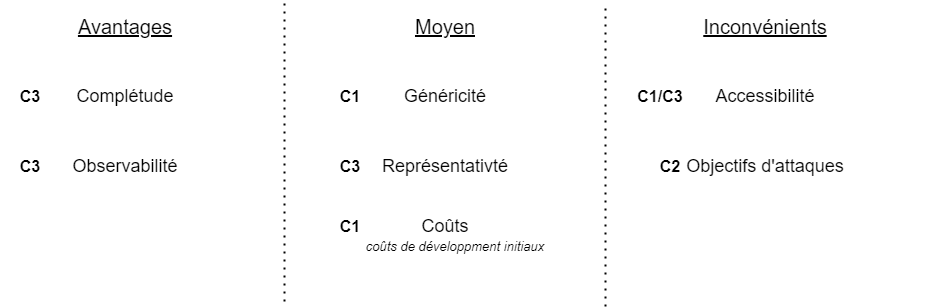
\includegraphics[scale=.43]{ch2-background/img/advantages-formal.drawio.png}
              \caption{Caractéristiques des méthodes formelles}
              \label{fig:soa-tools-scheme-formal}
            \end{figure}
            
            La figure \ref{fig:soa-tools-scheme-simu} présente les caractéristiques des outils basés sur les méthodes formelles.
            Les méthodes formelles ont un avantage en ce qui concerne la complétude des résultats, dépendant de la technique utilisée. 
            Ces approches étant appliquées à des niveaux variés d'abstraction, et donc de modèles de faute, la représentativité des
            résultats est très variable.
            La performance n'est pas réellement comparable par rapport aux outils basés sur les tests, puisque tous les chemins et toutes les combinaisons de fautes sont potentiellement explorés, mais certains outils souffrent d'un problème de passage à l'échelle, corrélé à la méthode formelle utilisée.
            L'accessibilité et l'automatisation ne sont pas toujours bons pour ces outils, demandant parfois une expertise de l'utilisateur dans la méthode formelle utilisée ou bien une intervention importante de la part de l'utilisateur \cite{Larsson/VERIFY07}.
    
        \subsection{Conclusion}
        \label{sec:soa-tools-conclusion}
            
            Des approches très variées ont été proposées pour l'évaluation de la robustesse dans le cadre de l'injection de fautes, comme l'ont montré les sections précédentes.
            
                \begin{table}[h]
                    {\small
                    \begin{center}
                    \setlength\tabcolsep{3.5pt}
                        \begin{tabular}{|l|c|c|c|c|}
                        \hline
                        Méthode & Mise-en-place & Représentativité & Reproductibilité & Observabilité  \\ \hline
                        Injection Physique & Très élevé & Très élevé & Faible - Elevé & Faible  \\ \hline
                        SWIFI & Faible & Faible - élevé & Moyen & Moyen  \\ \hline
                        Simulation & Faible elevé & Moyen - élevé & Elevé & Elevé - Très élevé  \\ \hline
                        Méthodes formelles & Faible - Elevé & Moyen - élevé & Moyen - elevé & Elevé - Très élevé  \\ \hline
                        \end{tabular}
                        
                        \vspace{0.2cm}
                        
                        \begin{tabular}{|l|c|c|c|c|c|}
                        \hline
                        Méthode & Contexte  & Complétude & Accessibilité & Généricité & Contexte \\ \hline
                        Inj Physique & Varié &Faible & Faible & Faible & Varié \\ \hline
                        Swifi & Varié & Faible & Moyen & Elevée & Varié \\ \hline
                        Simu & Varié & Faible & Moyen & Moyen - élevé & Varié \\ \hline
                        Formal & Limité & Elevé - Très élevé & Faible & Moyen - élevé & Limité \\ \hline
                        \end{tabular}
                    \end{center}
                    }           
                    \caption{Comparaison des méthodes d'analyse de robustesse contre les fautes \label{tbl:tools-conclusion}}
                \end{table}
            
            La table \ref{tbl:tools-conclusion} compare les caractéristiques de la section \ref{sec:soa-tools-carac} pour les différentes techniques d'analyse présentées dans les sections précédentes.
            Chaque valeur correspond à une pondération entre \textit{faible}, \textit{moyen}, \textit{élevé} et \textit{très élevé}, visant à préserver les rapports entre les classes de techniques d'analyse ainsi que les variations au sein d'une même classe.
            
            Les méthodes formelles ont un très net avantage en ce qui concerne la couverture des exécutions fautées, mais certaines techniques comme l'exécution symbolique souffrent de l'explosion combinatoire induite par les fautes pour le passage à l'échelle, en particulier dans un contexte multi-fautes.
            De plus, certaines propriétés et objectif d'attaque peuvent être difficiles à exprimer ou à analyser avec certaines approches formelles, notamment les propriétés basées sur la comparaisons de traces (canaux-auxiliaires) qui peuvent être plus simples à évaluer avec un golden run. 
            La simulation offre des avantages en termes de contrôlabilité.
            Les méthodes de type \gls{swifi} sont généralement les plus faciles à mettre en place.
            
            Certaines caractéristiques dépendent fortement des choix de conception et d'implémentation de l'outil. Si la contrôlabilité est difficile dans le cadre de l'injection physique, cette caractéristique dépend surtout de ce que l'outil met à disposition à l'utilisateur pour les autres classes d'outils, les outils simulant un système (que ce soit dans un simulateur ou par une modélisation formelle) étant aussi avantagés. 
            L'accessibilité est un bon exemple de caractéristique dépendant en grande partie de l'outil plus que de la méthode utilisée, qu'il s'agisse d'automatisation, de contrôlabilité ou d'expertise. 
            
            D'autres caractéristiques dépendent aussi fortement du niveau de représentation considéré par l'outil, qui peut être très variable au sein des outils d'une même méthode d'analyse. 
            Dans ce cas, le niveau de représentation de l'outil influe directement sur la représentativité, les modèles de faute supportés et la généricité de l'outil.
            
            L'outil Lazart, qui est l'objet du chapitre suivant, est un outil d'analyse formelle utilisant l'exécution dynamique-symbolique.
            Lazart utilise l'outil KLEE qui effectue une exécution dynamique-symbolique sur le code \gls{llvm} et peut ainsi être vu comme un simulateur utilisant un modèle mémoire et une représentation du système particuliers.
            Les fautes sont introduites par une mutation du programme fourni à KLEE, correspondant à ce qui existe dans le cadre des outils \gls{swifi} au niveau \gls{llvm}.
            
            Lazart vise à répondre à certaines problématiques tirées de cette section en ce qui concerne ce type d'outils reposant sur les méthodes formelle ainsi que l'émulation des fautes au niveau logiciel.
            
            \begin{itemize}
                \item \textit{Performance} et \textit{passage à l'échelle}: maîtriser le multi-fautes et l'explosion combinatoire engendrée.
                \item \textit{Représentativité}: limiter la perte de représentativité liée à la sur-couche de l'émulation des fautes.
                \item \textit{Accessibilité} et \textit{généricité}: limiter le niveau d'expertise requis pour l'utilisation de l'outil et laisser une contrôlabilité élevée à l'utilisateur.
            \end{itemize}
            
            Les contributions de Lazart visent ainsi à proposer des solutions pour ces problématiques:
            \begin{itemize}
                \item Support de l'inter-procédural et de la combinaison de modèles de faute ainsi qu'une description à grain fin des fautes par l'utilisateur (\textit{représentativité} et \textit{contrôlabilité}).
                \item Une \gls{api} Python facilitant la description des analyses et la présentation des résultats (\textit{accessibilité}).
                \item Une analyse plus fine des résultats produits.
            \end{itemize}